\documentclass[../DoAn.tex]{subfiles}
\begin{document}

Tiếp nối Chương 3, nơi các nền tảng công nghệ và cơ sở lý thuyết đã được phân tích, Chương 4 tập trung hiện thực hóa các lựa chọn đó thành kiến trúc phần mềm, thiết kế dữ liệu, giao diện và quy trình triển khai cụ thể của hệ thống marketplace đa nhà bán hàng. Nội dung chương lần lượt trình bày về: thiết kế kiến trúc và biểu đồ gói của hệ thống trong phần \ref{section:4.1}; thiết kế chi tiết giao diện, mô-đun nghiệp vụ và cơ sở dữ liệu trong phần \ref{section:4.2}; quá trình xây dựng ứng dụng cùng các công cụ, thư viện và kết quả đạt được trong phần \ref{section:4.3}; kiểm thử hệ thống trong phần \ref{section:4.4}; và sau cùng là mô hình triển khai thực tế của đồ án trong phần \ref{section:4.5}.

% ─── SECTION 1: THIẾT KẾ KIẾN TRÚC ─────────────────────────────────────────
\section{Thiết kế kiến trúc}
\label{section:4.1}

\subsection{Lựa chọn kiến trúc phần mềm}
Đồ án lựa chọn kiến trúc web nhiều tầng theo định hướng MERN Stack với hai nền tảng độc lập: ứng dụng giao diện người dùng (frontend) viết bằng React 19 và máy chủ xử lý nghiệp vụ (backend) viết bằng Node.js/Express 5. Hai nền tảng giao tiếp qua giao thức REST trên HTTPS; kênh sự kiện thời gian thực được tách riêng thông qua Socket.IO (WebSocket).

\textbf{Kiến trúc phân lớp phía máy chủ.} Thay vì phát triển theo hướng vi dịch vụ ngay từ đầu, backend được hiện thực dưới dạng một máy chủ Express duy nhất nhưng phân tách nội bộ thành bốn tầng rõ ràng:

(i) \textit{Tầng định tuyến} (\texttt{routes/}): tiếp nhận yêu cầu HTTP, áp dụng middleware xác thực JWT và giới hạn tần suất, rồi chuyển tiếp đến Controller tương ứng.

(ii) \textit{Tầng điều phối} (\texttt{controllers/}): phân giải tham số từ đối tượng \texttt{Request}, gọi Service và trả phản hồi JSON chuẩn hóa về client.

(iii) \textit{Tầng nghiệp vụ} (\texttt{services/}): chứa toàn bộ logic xử lý, bao gồm tính toán giá, quản lý tồn kho, phiên xác thực và giao tiếp với các dịch vụ bên ngoài (Stripe, VNPay, Cloudinary).

(iv) \textit{Tầng dữ liệu} (\texttt{models/}): định nghĩa schema Mongoose và trừu tượng hóa tương tác với MongoDB.

Nguyên tắc thiết kế quan trọng là các tầng chỉ phụ thuộc theo một chiều từ trên xuống dưới: Route phụ thuộc Controller, Controller phụ thuộc Service, Service phụ thuộc Model. Không tầng nào phụ thuộc ngược hoặc bỏ qua tầng kế tiếp.

\textbf{Kiến trúc thành phần phía giao diện.} Frontend áp dụng kiến trúc thành phần (Component-Based Architecture) đặc trưng của React, được tổ chức theo mô hình phân cấp bốn tầng: Pages (màn hình chính), Components (thành phần giao diện tái sử dụng), Context và Hooks (quản lý trạng thái và logic nghiệp vụ phía client), Utils (hàm tiện ích định dạng).

\textbf{Lý do không chọn Microservices.} Dù kiến trúc Microservices mang lại khả năng mở rộng độc lập theo từng dịch vụ, phạm vi đồ án là hệ thống thương mại điện tử một cụm máy chủ với lưu lượng vừa phải. Kiến trúc nguyên khối phân lớp giảm đáng kể chi phí vận hành, đơn giản hóa giao dịch nguyên tử giữa các nghiệp vụ (đặt hàng và giữ kho), đồng thời phù hợp với quy mô phát triển của một nhóm nhỏ. Cách phân chia mã nguồn hiện tại vẫn đủ tách biệt để có thể tách thành vi dịch vụ trong giai đoạn sau nếu cần thiết.

\subsection{Thiết kế tổng quan}
\label{section:4.1.2}

Hình \ref{fig:architecture_overview} mô tả kiến trúc triển khai tổng thể của hệ thống. Phía khách hàng truy cập ứng dụng mua sắm xây dựng bằng React + Vite; phía đối tác bán hàng sử dụng một ứng dụng React độc lập để quản trị sản phẩm, đơn hàng, voucher và thống kê. Cả hai giao diện cùng giao tiếp với backend Express thông qua REST API, trong đó luồng chat thời gian thực sử dụng Socket.IO còn thông báo trên dashboard vendor sử dụng Server-Sent Events (SSE).

\begin{figure}[htbp]
    \centering
    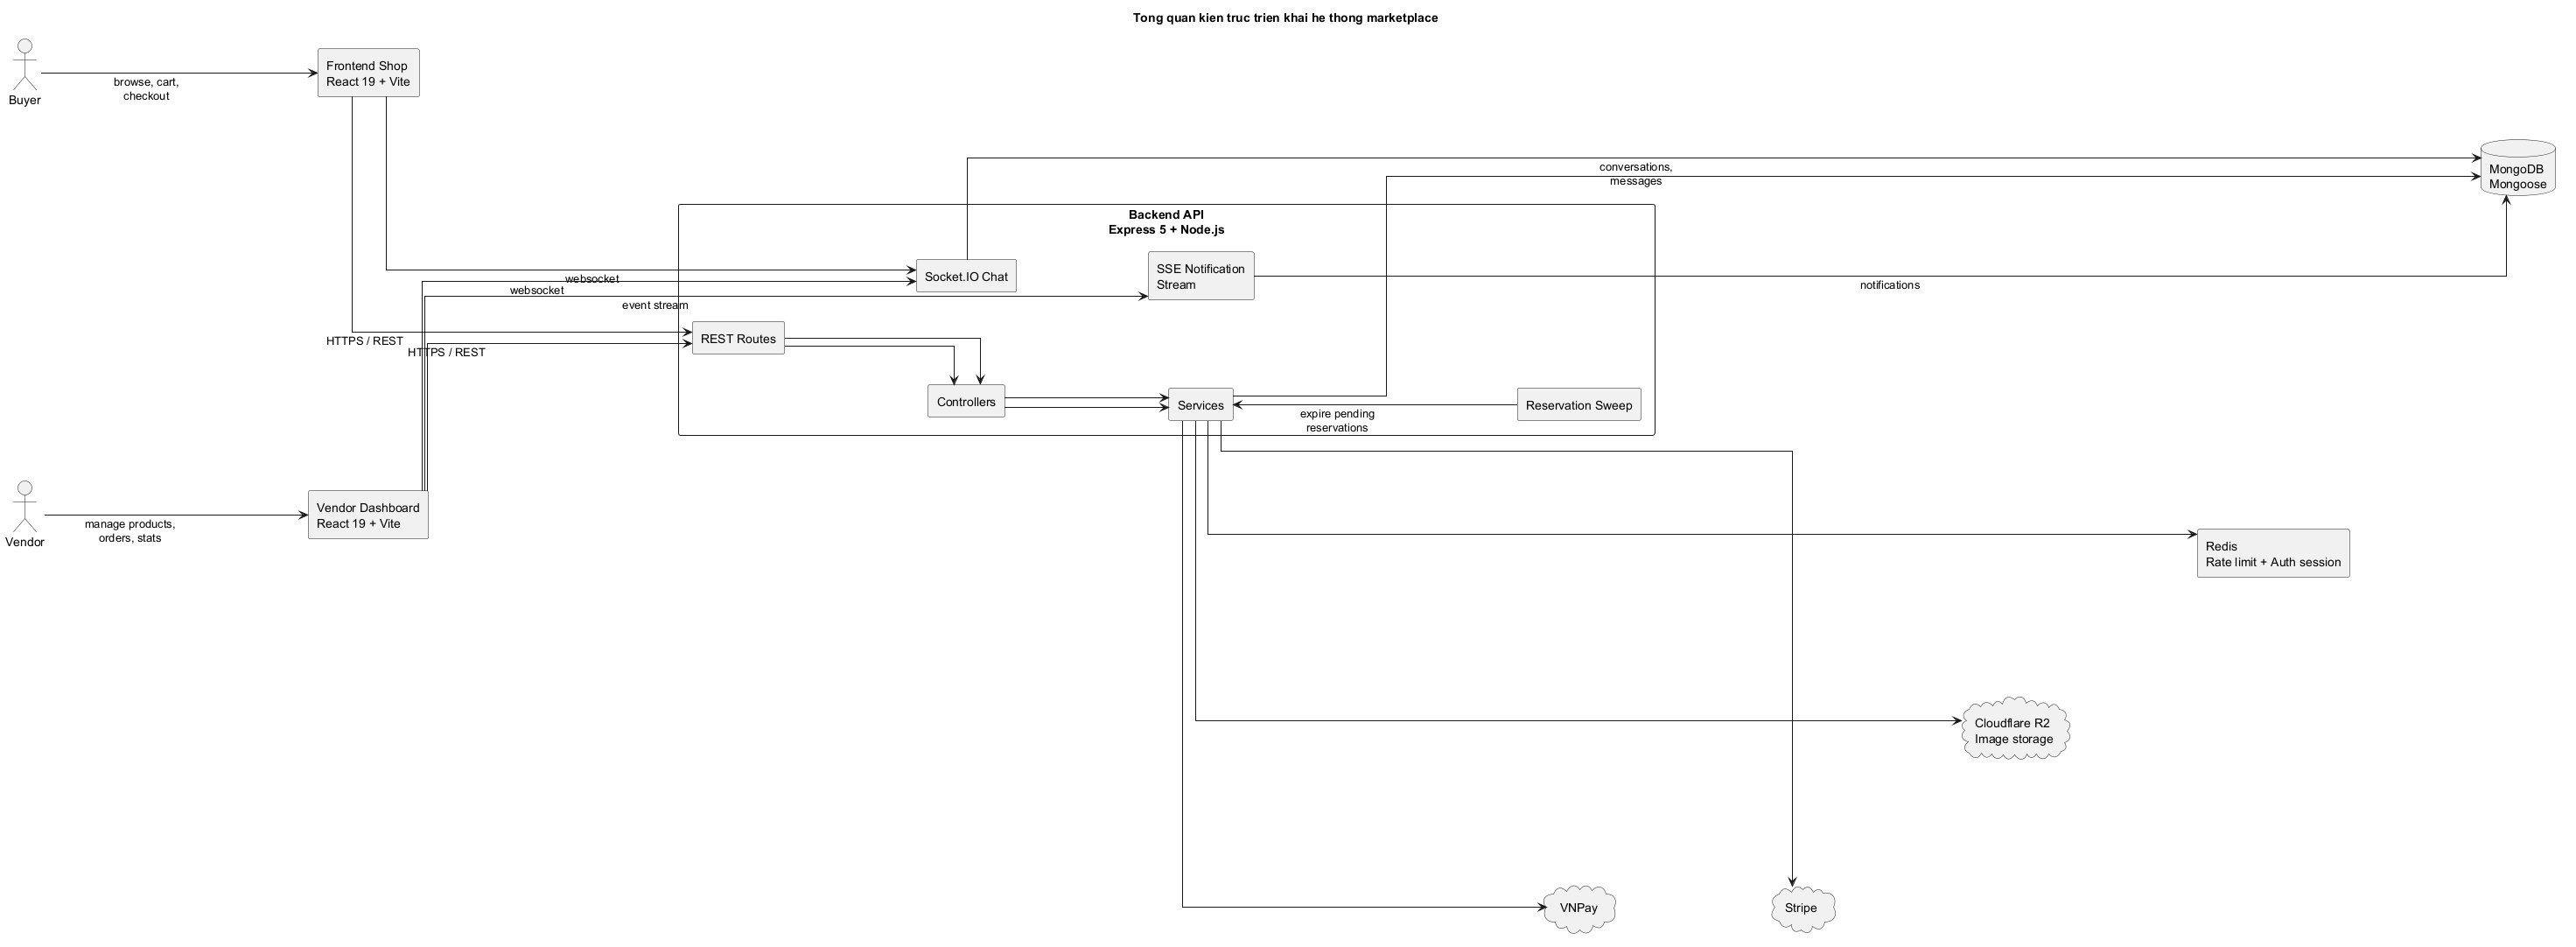
\includegraphics[width=0.98\textwidth,height=0.78\textheight,keepaspectratio]{images/generated/architecture_overview.png}
    \caption{Kiến trúc triển khai tổng thể của hệ thống marketplace}
    \label{fig:architecture_overview}
\end{figure}

Biểu đồ gói phía máy chủ trong Hình \ref{fig:be_package} trình bày sáu gói chính của backend với phụ thuộc một chiều từ ngoài vào trong. Gói \texttt{routes} phụ thuộc vào \texttt{middleware} và \texttt{controllers}; \texttt{controllers} phụ thuộc \texttt{services} và \texttt{utils}; \texttt{services} phụ thuộc \texttt{models} và \texttt{config}. Hai gói ngoại vi là \texttt{models} (kết nối MongoDB) và \texttt{config} (cấu hình Redis, Cloudflare R2) không phụ thuộc bất kỳ gói nghiệp vụ nào.

\begin{figure}[htbp]
    \centering
    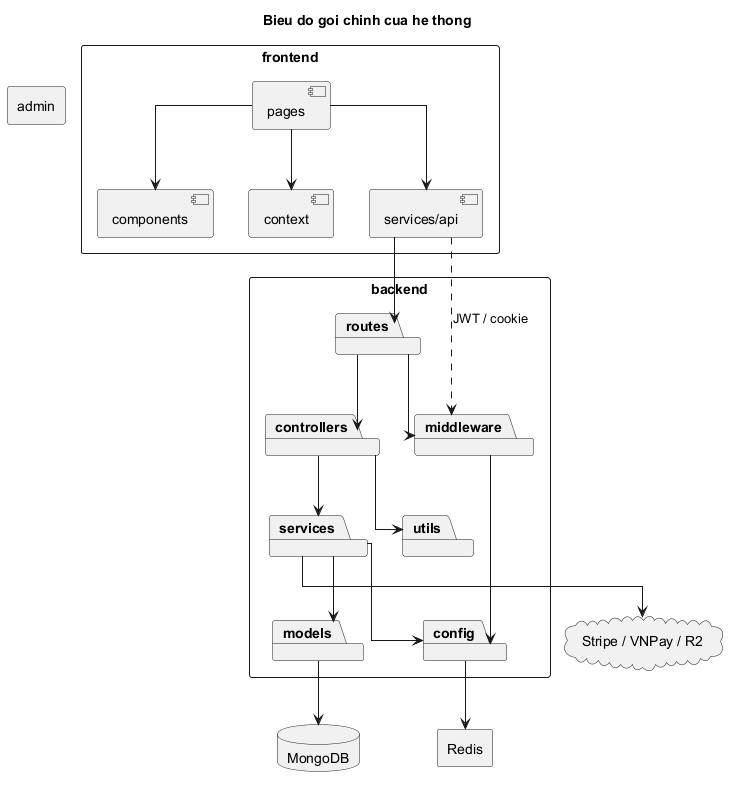
\includegraphics[width=0.95\textwidth,height=0.78\textheight,keepaspectratio]{images/generated/backend_package_diagram.png}
    \caption{Biểu đồ gói phía máy chủ}
    \label{fig:be_package}
\end{figure}

Biểu đồ gói phía giao diện trong Hình \ref{fig:fe_package} cho thấy gói \texttt{pages} sử dụng \texttt{components} để dựng giao diện, tiêu thụ trạng thái từ \texttt{context} và gọi logic nghiệp vụ thông qua \texttt{hooks}. Gói \texttt{hooks} là cầu nối giữa tầng hiển thị và tầng gọi API: hook đọc/ghi trạng thái trong \texttt{context} và gửi yêu cầu qua gói \texttt{api}. Gói \texttt{utils} cung cấp các hàm tiện ích thuần túy và không phụ thuộc bất kỳ gói nào khác.

\begin{figure}[htbp]
    \centering
    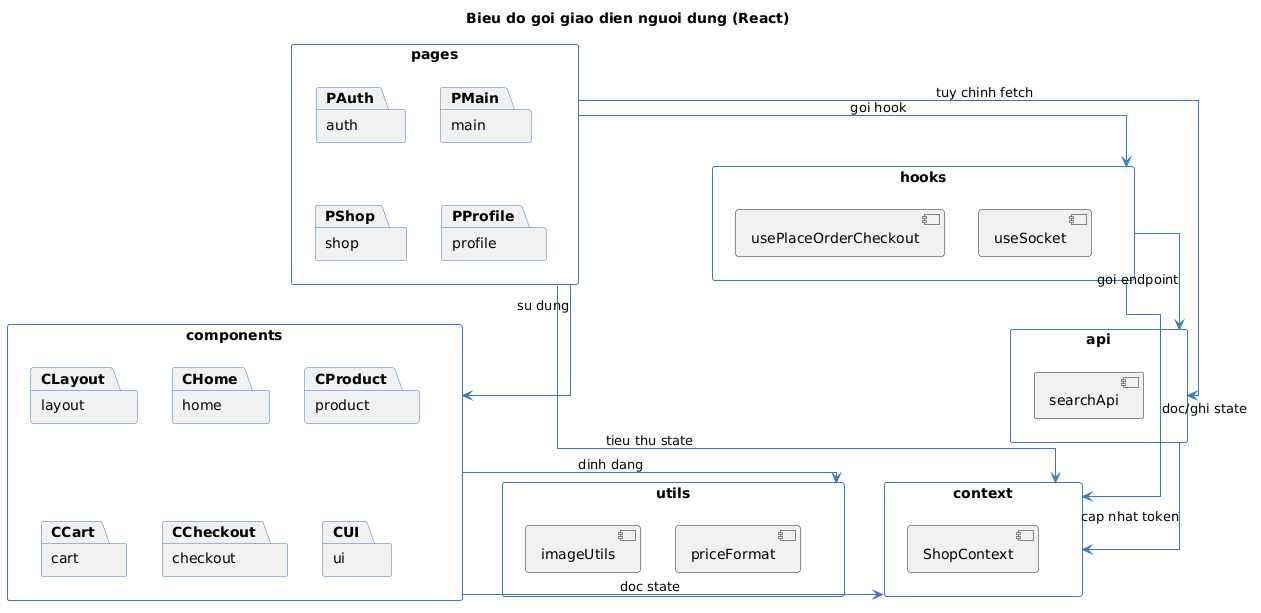
\includegraphics[width=0.85\textwidth]{images/generated/frontend_package_diagram.png}
    \caption{Biểu đồ gói phía giao diện (Frontend)}
    \label{fig:fe_package}
\end{figure}

\subsection{Thiết kế chi tiết gói}

\textbf{Gói \texttt{routes} và \texttt{middleware}.} Mỗi nhóm nghiệp vụ được ánh xạ thành một tệp route riêng biệt (ví dụ \texttt{productRoute.js}, \texttt{orderRoute.js}, \texttt{voucherRoute.js}). Middleware xác thực JWT (\texttt{auth.js}) và middleware phân quyền nhà bán hàng (\texttt{vendorAuth.js}) được áp dụng có chọn lọc trên từng route thay vì toàn cục, nhằm đảm bảo các endpoint công khai (tra cứu sản phẩm, danh mục) không cần xác thực.

\textbf{Gói \texttt{controllers}.} Mỗi controller giữ vai trò điều phối mỏng: phân giải tham số đầu vào từ \texttt{req.body}/\texttt{req.params}/\texttt{req.query}, gọi đúng hàm Service, xử lý ngoại lệ và trả phản hồi JSON. Controller không chứa logic nghiệp vụ hay truy vấn cơ sở dữ liệu trực tiếp.

\textbf{Gói \texttt{services}.} Đây là gói trung tâm của kiến trúc. Mỗi miền nghiệp vụ có một tệp Service tương ứng. Trong đó \texttt{voucherService.js} xử lý tính giá nhiều lớp, \texttt{orderService.js} điều phối giữ kho và giao dịch, \texttt{authSessionService.js} quản lý vòng đời phiên làm việc trên Redis, và \texttt{searchService.js} thực hiện tìm kiếm kết hợp từ khóa với điểm phù hợp cá nhân hóa. Mối quan hệ giữa các Service chủ đạo được thể hiện trong Hình \ref{fig:svc_class}.

\begin{figure}[htbp]
    \centering
    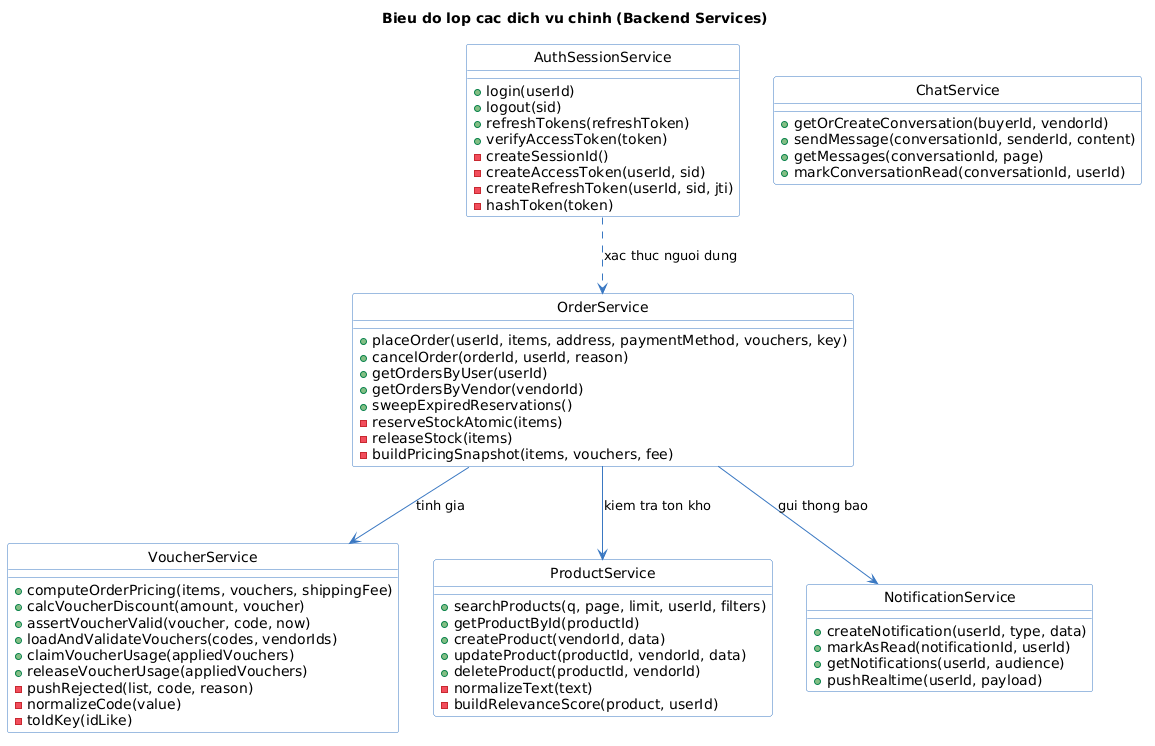
\includegraphics[width=0.95\textwidth]{images/generated/service_class_diagram.png}
    \caption{Biểu đồ lớp các dịch vụ chính phía máy chủ}
    \label{fig:svc_class}
\end{figure}

\textbf{Gói \texttt{context} và \texttt{hooks} (Frontend).} \texttt{ShopContext} lưu trữ tập trung các trạng thái toàn cục gồm danh sách sản phẩm hiển thị, nội dung giỏ hàng, thông tin người dùng đang đăng nhập và token xác thực. Hook \texttt{usePlaceOrderCheckout} đóng gói toàn bộ quy trình thanh toán gồm kiểm tra form, tính toán bảng giá và gọi endpoint đặt hàng, tách biệt logic này hoàn toàn khỏi thành phần giao diện.

% ─── SECTION 2: THIẾT KẾ CHI TIẾT ──────────────────────────────────────────
\section{Thiết kế chi tiết}
\label{section:4.2}

\subsection{Thiết kế giao diện}
Hệ thống giao diện được phát triển theo mô hình SPA với hai ứng dụng độc lập dùng chung định hướng thiết kế. Ứng dụng \texttt{frontend} phục vụ khách hàng cuối gồm các nhóm màn hình: trang chủ, danh sách sản phẩm, trang chi tiết sản phẩm, giỏ hàng, đặt hàng, theo dõi đơn, hồ sơ cá nhân, chat và thông báo. Ứng dụng vendor dashboard phục vụ đối tác bán hàng gồm các màn hình quản lý sản phẩm, đơn hàng, voucher, thống kê và chat.

\textbf{Đặc tả màn hình.} Giao diện được thiết kế theo phương pháp \textit{mobile-first responsive}: bố cục một cột trên màn hình từ 360px, hai cột trên màn hình máy tính bảng từ 768px và nhiều cột linh hoạt trên màn hình máy tính từ 1280px trở lên. Hệ thống bố cục sử dụng Tailwind CSS 3.4 với lưới 12 cột.

\textbf{Hệ màu và chuẩn tương tác.} Màu chủ đạo là cam (\texttt{\#F97316}) cho các phần tử tương tác và kêu gọi hành động; màu phụ là xám trung tính cho văn bản thứ yếu và trắng cho nền vùng nội dung. Hệ thống thống nhất ba quy tắc giao diện: thông báo phản hồi hiển thị dưới dạng toast góc dưới-phải qua React Toastify; hộp thoại xác nhận thao tác nguy hiểm dùng modal phủ toàn màn hình; trạng thái đang tải hiển thị skeleton placeholder.

Sơ đồ điều hướng chính của hai ứng dụng giao diện được minh họa trong Hình \ref{fig:ui_navigation_map}. Người mua đi từ khám phá sản phẩm đến giỏ hàng, đặt hàng và theo dõi đơn; vendor di chuyển chủ yếu giữa danh sách sản phẩm, đơn hàng, voucher, thống kê và chat.

\begin{figure}[htbp]
    \centering
    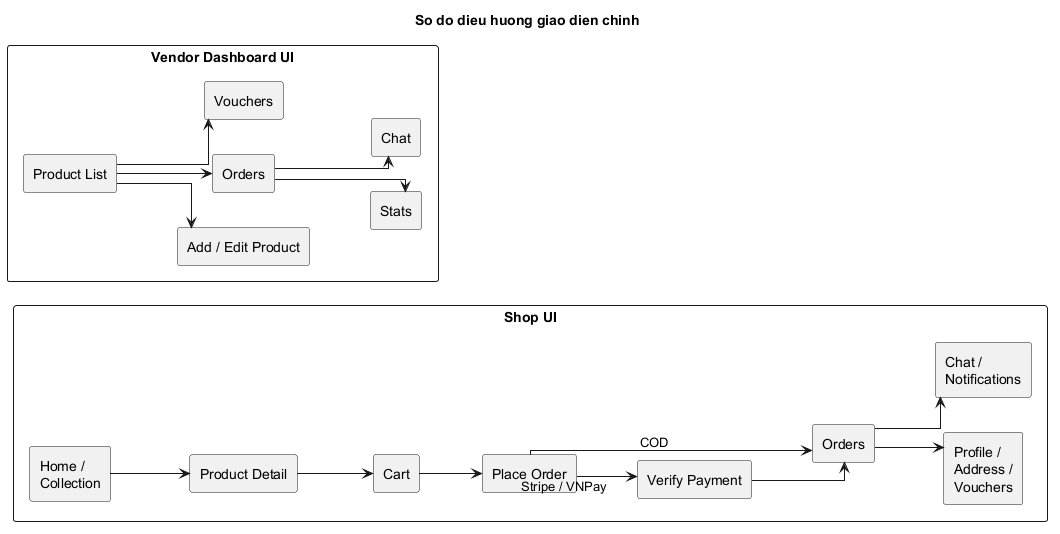
\includegraphics[width=0.96\textwidth,height=0.76\textheight,keepaspectratio]{images/generated/ui_navigation_map.png}
    \caption{Sơ đồ điều hướng giao diện chính của hệ thống}
    \label{fig:ui_navigation_map}
\end{figure}

\subsection{Thiết kế lớp}

\textbf{Các lớp nghiệp vụ chủ đạo.} Bốn đối tượng nghiệp vụ quan trọng nhất là \texttt{User}, \texttt{Product}, \texttt{Order} và \texttt{Voucher}. \texttt{User} giữ thông tin tài khoản hợp nhất cho cả người mua và người bán, phân biệt bằng trường \texttt{role}, giúp đơn giản hóa luồng xác thực. \texttt{Product} hỗ trợ cấu trúc phân cấp danh mục ba tầng, tập thuộc tính và biến thể SKU với tồn kho riêng từng SKU. \texttt{Order} ngoài các trường giao dịch cơ bản còn bổ sung \texttt{idempotencyKey}, \texttt{stockReservedAt}, \texttt{reservationExpiresAt} và dữ liệu cổng thanh toán để hỗ trợ giữ kho và thanh toán online an toàn. \texttt{Voucher} hỗ trợ ba kiểu \texttt{SHOP}, \texttt{PLATFORM} và \texttt{SHIPPING} với hai kiểu giảm giá phần trăm và số tiền cố định.

Mối quan hệ điều phối giữa các Service lớp đã được trình bày trong Hình \ref{fig:svc_class}. \texttt{OrderService} đóng vai trò điều phối trung tâm: khi đặt hàng nó gọi \texttt{VoucherService.computeOrderPricing()} để tính bảng giá nhiều lớp, gọi giữ kho nguyên tử thông qua \texttt{ProductService} và kích hoạt \texttt{NotificationService.pushRealtime()} để thông báo cho nhà bán hàng.

\textbf{Biểu đồ tuần tự: Tạo đơn hàng.} Hình \ref{fig:seq_order} mô tả luồng tạo đơn hàng với cơ chế kiểm soát trùng lệnh và giữ kho nguyên tử. Sau khi client gửi yêu cầu kèm mã định danh chống trùng đơn, backend tra cứu đơn cũ trước; nếu chưa tồn tại, hệ thống thực hiện giữ kho bằng phép cập nhật có điều kiện ($\$inc$ kết hợp điều kiện số lượng đủ) để ngăn bán vượt tồn kho đồng thời. Thông tin thời điểm và thời hạn giữ kho được lưu vào bản ghi đơn hàng để tác vụ nền có thể hoàn trả nếu thanh toán quá hạn.

\begin{figure}[htbp]
    \centering
    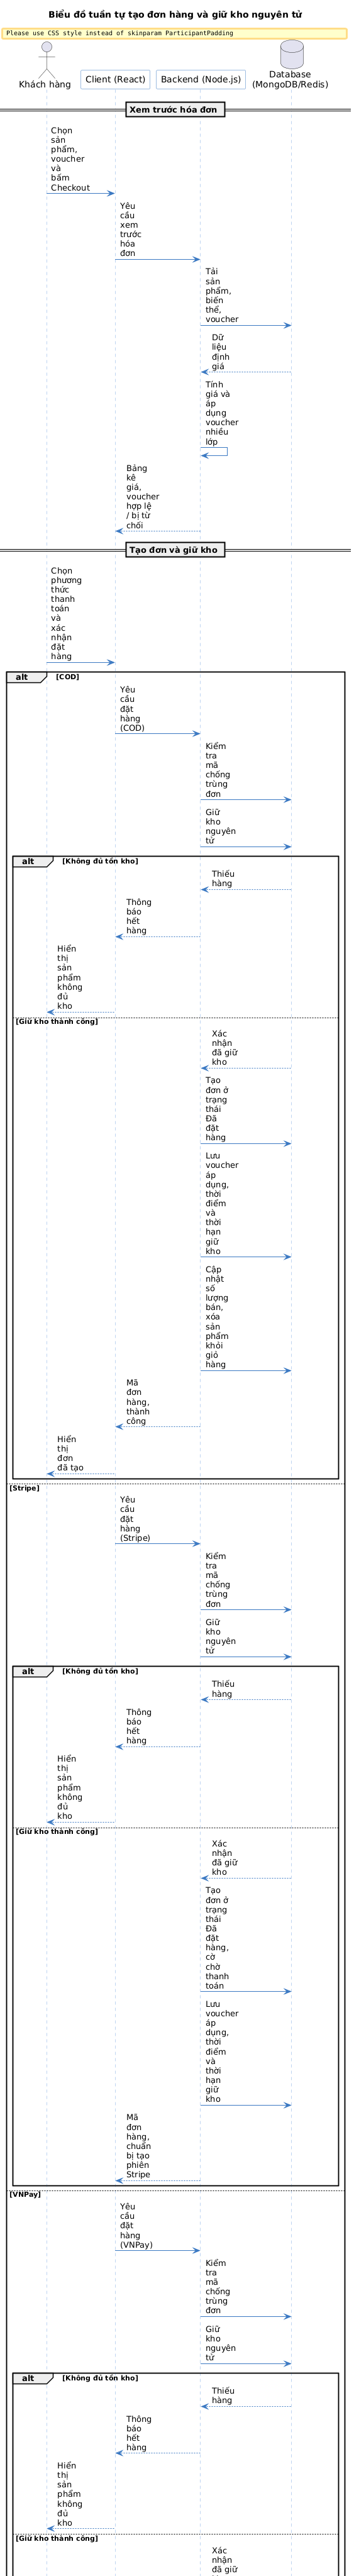
\includegraphics[width=0.92\textwidth,height=0.78\textheight,keepaspectratio]{images/generated/order_creation_sequence.png}
    \caption{Biểu đồ tuần tự luồng tạo đơn hàng và giữ kho nguyên tử}
    \label{fig:seq_order}
\end{figure}

\textbf{Biểu đồ tuần tự: Xác nhận thanh toán trực tuyến.} Hình \ref{fig:seq_payment} mô tả hai kịch bản thanh toán trực tuyến (Stripe và VNPay) và cơ chế tự động hủy đơn quá hạn. Với Stripe, kết quả thanh toán được truyền về qua webhook; với VNPay, kết quả truyền qua URL callback có chữ ký số. Tác vụ nền chạy theo chu kỳ phát hiện đơn chưa thanh toán đã quá thời hạn giữ kho, tự động chuyển trạng thái sang đã hủy và hoàn trả tồn kho cùng lượt sử dụng voucher.

\begin{figure}[htbp]
    \centering
    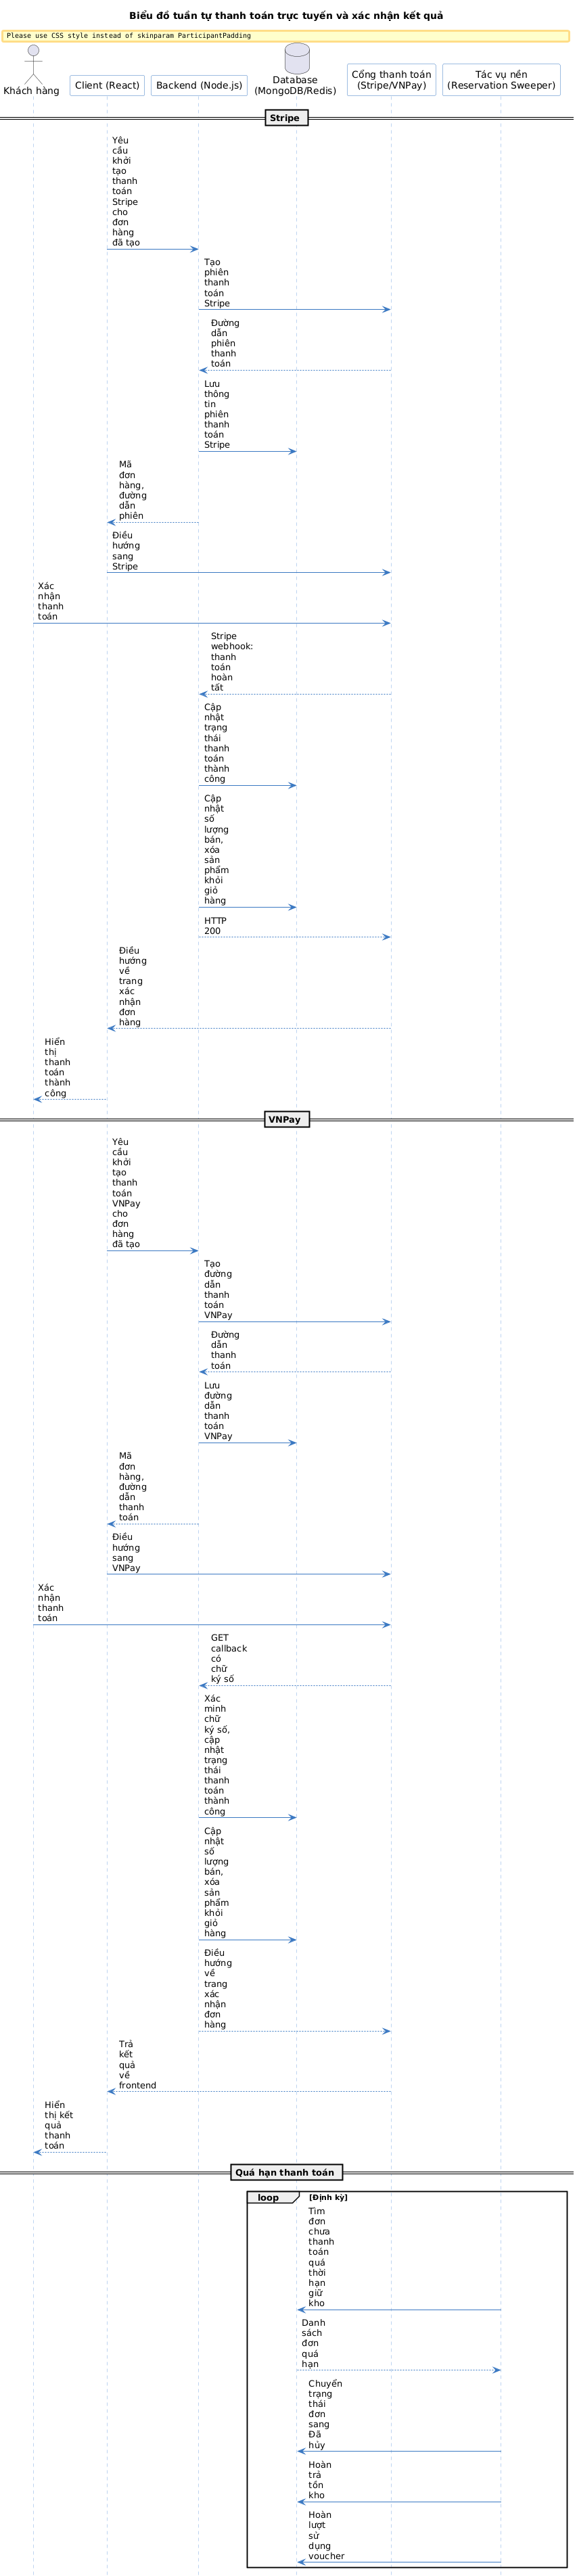
\includegraphics[width=0.92\textwidth,height=0.78\textheight,keepaspectratio]{images/generated/online_payment_confirmation_sequence.png}
    \caption{Biểu đồ tuần tự xác nhận thanh toán trực tuyến}
    \label{fig:seq_payment}
\end{figure}

\subsection{Thiết kế cơ sở dữ liệu}
Mô hình dữ liệu chính của hệ thống được thể hiện trong Hình \ref{fig:marketplace_er_diagram}. Dù triển khai trên MongoDB, sơ đồ vẫn được trình bày theo kiểu thực thể liên kết để làm rõ các quan hệ nghiệp vụ cốt lõi giữa người dùng, sản phẩm, đơn hàng, voucher, đánh giá, tương tác và hội thoại.

\begin{figure}[htbp]
    \centering
    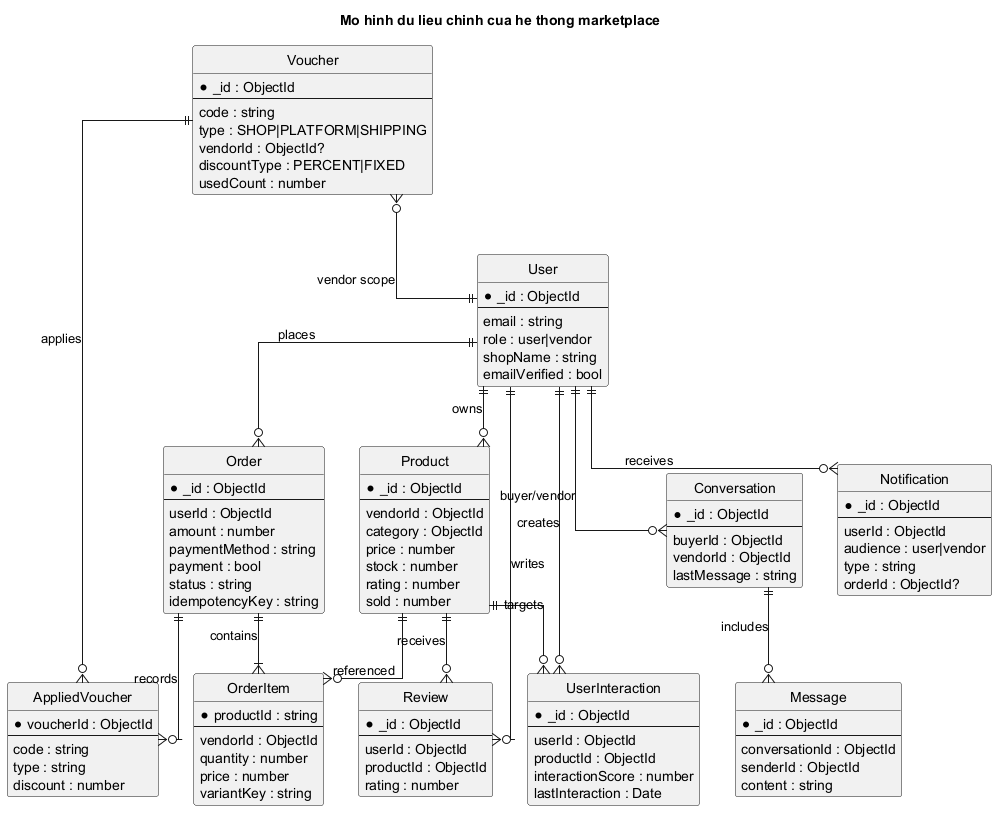
\includegraphics[width=0.98\textwidth,height=0.84\textheight,keepaspectratio]{images/generated/marketplace_er_diagram.png}
    \caption{Mô hình dữ liệu chính của hệ thống marketplace}
    \label{fig:marketplace_er_diagram}
\end{figure}

Lược đồ dữ liệu được thiết kế theo hướng kết hợp giữa tham chiếu và nhúng tài liệu. Các tài liệu có vòng đời độc lập như \texttt{user}, \texttt{product}, \texttt{voucher}, \texttt{review}, \texttt{notification} hay \texttt{conversation} được tách thành các collection riêng. Trong khi đó, các cấu phần gắn chặt với đơn hàng như \texttt{items}, \texttt{appliedVouchers} và thông tin theo vendor được nhúng trực tiếp vào tài liệu \texttt{order} để giảm số lần join logic ở tầng ứng dụng và bảo toàn trạng thái giao dịch theo thời điểm đặt hàng.

Về tối ưu truy vấn, collection \texttt{product} có chỉ mục văn bản trên \texttt{name}, \texttt{brand} và \texttt{tags} để phục vụ tìm kiếm server-side. Collection \texttt{order} có chỉ mục duy nhất trên cặp \texttt{userId} và \texttt{idempotencyKey} để chặn tạo đơn trùng. Collection \texttt{userInteraction} có chỉ mục kết hợp \texttt{userId}~--~\texttt{productId} nhằm bảo đảm mỗi người dùng chỉ có một hồ sơ tương tác cho một sản phẩm.

Cấu trúc các collection quan trọng nhất được trình bày chi tiết từ Bảng \ref{table:schema_user} đến Bảng \ref{table:schema_interaction}.

\begin{table}[htbp]
    \centering
    \caption{Cấu trúc collection \texttt{users} (Người dùng và nhà bán hàng)}
    \label{table:schema_user}
    \begin{tabular}{|l|l|l|p{7.5cm}|}
        \hline
        \textbf{Trường dữ liệu} & \textbf{Kiểu} & \textbf{Ràng buộc} & \textbf{Mô tả} \\ \hline
        \texttt{\_id} & ObjectId & Khóa chính & Định danh duy nhất của người dùng. \\ \hline
        \texttt{name} & String & Required & Họ và tên người dùng. \\ \hline
        \texttt{email} & String & Unique, Required & Địa chỉ email dùng để đăng nhập. \\ \hline
        \texttt{password} & String & Select: false & Mật khẩu đã được mã hóa bằng bcrypt. \\ \hline
        \texttt{role} & String & Default: 'user' & Vai trò: \texttt{'user'} hoặc \texttt{'vendor'}. \\ \hline
        \texttt{avatar} & Object & -- & Đường dẫn ảnh gốc và ảnh thu nhỏ (thumbnail). \\ \hline
        \texttt{cartData} & Object & Default: \{\} & Giỏ hàng lưu tạm của khách hàng. \\ \hline
        \texttt{shopName} & String & -- & Tên gian hàng (chỉ dành cho vendor). \\ \hline
        \texttt{emailVerified} & Boolean & Default: false & Trạng thái xác thực email. \\ \hline
    \end{tabular}
\end{table}

\begin{table}[htbp]
    \centering
    \caption{Cấu trúc collection \texttt{products} (Sản phẩm)}
    \label{table:schema_product}
    \begin{tabular}{|l|l|l|p{7.5cm}|}
        \hline
        \textbf{Trường dữ liệu} & \textbf{Kiểu} & \textbf{Ràng buộc} & \textbf{Mô tả} \\ \hline
        \texttt{\_id} & ObjectId & Khóa chính & Định danh duy nhất của sản phẩm. \\ \hline
        \texttt{name} & String & Required & Tên sản phẩm (chỉ mục text). \\ \hline
        \texttt{price} & Number & Required & Giá bán cơ bản. \\ \hline
        \texttt{stock} & Number & Default: 0 & Số lượng tồn kho cơ bản. \\ \hline
        \texttt{category} & ObjectId & Ref: category & Danh mục cấp 1 của sản phẩm. \\ \hline
        \texttt{vendorId} & ObjectId & Ref: user & Định danh vendor sở hữu sản phẩm. \\ \hline
        \texttt{sold} & Number & Default: 0 & Số lượng sản phẩm đã bán. \\ \hline
        \texttt{rating} & Number & Default: 0 & Điểm đánh giá trung bình (1--5). \\ \hline
        \texttt{attributes} & Array & -- & Tập thuộc tính (tên và danh sách giá trị). \\ \hline
        \texttt{variants} & Array & -- & Biến thể SKU (tổ hợp thuộc tính, giá và tồn kho riêng). \\ \hline
        \texttt{isActive} & Boolean & Default: true & Trạng thái kinh doanh của sản phẩm. \\ \hline
    \end{tabular}
\end{table}

\begin{table}[htbp]
    \centering
    \caption{Cấu trúc collection \texttt{orders} (Đơn hàng)}
    \label{table:schema_order}
    \begin{tabular}{|l|l|l|p{7.5cm}|}
        \hline
        \textbf{Trường dữ liệu} & \textbf{Kiểu} & \textbf{Ràng buộc} & \textbf{Mô tả} \\ \hline
        \texttt{\_id} & ObjectId & Khóa chính & Định danh duy nhất của đơn hàng. \\ \hline
        \texttt{userId} & ObjectId & Ref: user & Người mua hàng. \\ \hline
        \texttt{items} & Array & -- & Danh sách chi tiết các mặt hàng (snapshot tại thời điểm đặt). \\ \hline
        \texttt{pricing} & Object & -- & Bảng giá: subtotal, shopDiscount, platformDiscount, finalTotal. \\ \hline
        \texttt{paymentMethod} & String & Required & Phương thức: \texttt{'COD'}, \texttt{'Stripe'}, \texttt{'VNPay'}. \\ \hline
        \texttt{payment} & Boolean & Default: false & Trạng thái thanh toán thành công. \\ \hline
        \texttt{status} & String & Default: 'Order Placed' & Trạng thái vận chuyển của đơn hàng. \\ \hline
        \texttt{idempotencyKey} & String & Unique (cặp) & Khóa chống trùng lặp giao dịch đặt hàng. \\ \hline
        \texttt{reservationExpiresAt} & Number & -- & Thời gian hết hạn giữ kho. \\ \hline
        \texttt{vendors} & Array & -- & Danh sách chia nhỏ đơn theo từng shop để điều phối. \\ \hline
    \end{tabular}
\end{table}

\begin{table}[htbp]
    \centering
    \caption{Cấu trúc collection \texttt{vouchers} (Mã giảm giá)}
    \label{table:schema_voucher}
    \begin{tabular}{|l|l|l|p{7.5cm}|}
        \hline
        \textbf{Trường dữ liệu} & \textbf{Kiểu} & \textbf{Ràng buộc} & \textbf{Mô tả} \\ \hline
        \texttt{\_id} & ObjectId & Khóa chính & Định danh duy nhất của voucher. \\ \hline
        \texttt{code} & String & Unique, Required & Mã ký tự để áp dụng (viết hoa). \\ \hline
        \texttt{type} & String & Required & Loại: \texttt{'SHOP'}, \texttt{'PLATFORM'}, \texttt{'SHIPPING'}. \\ \hline
        \texttt{discountType} & String & Required & Kiểu giảm: \texttt{'PERCENT'} hoặc \texttt{'FIXED'}. \\ \hline
        \texttt{discountValue} & Number & Required & Giá trị giảm giá tương ứng. \\ \hline
        \texttt{minOrderValue} & Number & Default: 0 & Giá trị đơn hàng tối thiểu để áp dụng. \\ \hline
        \texttt{vendorId} & ObjectId & Ref: user & Cửa hàng áp dụng (chỉ dùng cho SHOP voucher). \\ \hline
        \texttt{usageLimit} & Number & Default: 0 & Giới hạn số lần sử dụng tối đa. \\ \hline
        \texttt{usedCount} & Number & Default: 0 & Số lần thực tế đã được dùng. \\ \hline
    \end{tabular}
\end{table}

\begin{table}[htbp]
    \centering
    \caption{Cấu trúc collection \texttt{userinteractions} (Tương tác người dùng)}
    \label{table:schema_interaction}
    \begin{tabular}{|l|l|l|p{7.5cm}|}
        \hline
        \textbf{Trường dữ liệu} & \textbf{Kiểu} & \textbf{Ràng buộc} & \textbf{Mô tả} \\ \hline
        \texttt{userId} & ObjectId & Ref: user & Định danh người dùng tương tác. \\ \hline
        \texttt{productId} & ObjectId & Ref: product & Định danh sản phẩm tương tác. \\ \hline
        \texttt{interactions} & Object & -- & Số lần viewed, clicked, addedToCart, purchased. \\ \hline
        \texttt{interactionScore} & Number & Default: 0 & Điểm số tương tác tổng hợp động. \\ \hline
        \texttt{lastInteraction} & Date & Default: Now & Mốc thời gian tương tác gần nhất. \\ \hline
        \texttt{decayFactor} & Number & Default: 1 & Hệ số suy hao thời gian (chu kỳ bán rã 30 ngày). \\ \hline
    \end{tabular}
\end{table}

% ─── SECTION 3: XÂY DỰNG ỨNG DỤNG ──────────────────────────────────────────
\section{Xây dựng ứng dụng}
\label{section:4.3}

\subsection{Thư viện và công cụ sử dụng}
Bảng \ref{table:tools_backend} và Bảng \ref{table:tools_frontend} tổng hợp các công cụ, thư viện và nền tảng chính được sử dụng trong quá trình xây dựng hệ thống. Các phiên bản được lấy trực tiếp từ các tệp \texttt{package.json} của dự án.

\begin{table}[htbp]
    \centering
    \caption{Thư viện và công cụ chính phía máy chủ}
    \label{table:tools_backend}
    \begin{tabular}{|p{2.8cm}|p{4.2cm}|p{2.2cm}|p{5.8cm}|}
        \hline
        \textbf{Nhóm} & \textbf{Công cụ / thư viện} & \textbf{Phiên bản} & \textbf{Vai trò sử dụng} \\ \hline
        Runtime & Node.js + Express & LTS / 5.1.0 & Xây dựng REST API, middleware và điều phối nghiệp vụ. \\ \hline
        Cơ sở dữ liệu & MongoDB + Mongoose & -- / 8.14.1 & Lưu trữ dữ liệu nghiệp vụ và định nghĩa lược đồ tài liệu. \\ \hline
        Cache / session & Redis & 4.7.1 & Giới hạn tần suất và quản lý phiên xác thực phía server. \\ \hline
        Xác thực & JWT + bcrypt & 9.0.2 / 5.1.1 & Ký token truy cập, refresh token rotation và băm mật khẩu. \\ \hline
        Thanh toán & Stripe & 18.1.0 & Tạo checkout session và xác minh thanh toán qua webhook. \\ \hline
        Ảnh sản phẩm & Cloudinary + Sharp & 2.6.0 / 0.34.5 & Upload ảnh sản phẩm và xử lý, nén ảnh trước khi lưu. \\ \hline
        Realtime & Socket.IO & 4.8.3 & Chat hai chiều giữa buyer và vendor. \\ \hline
        Kiểm thử & Jest + mongodb-memory-server & 30.3.0 / 11.0.1 & Kiểm thử đơn vị cho các service nghiệp vụ. \\ \hline
    \end{tabular}
\end{table}

\begin{table}[htbp]
    \centering
    \caption{Thư viện và công cụ chính phía giao diện và triển khai}
    \label{table:tools_frontend}
    \begin{tabular}{|p{2.8cm}|p{4.2cm}|p{2.2cm}|p{5.8cm}|}
        \hline
        \textbf{Nhóm} & \textbf{Công cụ / thư viện} & \textbf{Phiên bản} & \textbf{Vai trò sử dụng} \\ \hline
        UI framework & React + Vite & 19.0.0 / 6.2.0 & Xây dựng SPA cho khách hàng cuối. \\ \hline
        Điều hướng & React Router DOM & 7.5.0 & Quản lý route phía client. \\ \hline
        HTTP client & Axios & 1.9.0 & Gọi REST API với interceptor tự động làm mới token. \\ \hline
        WebSocket client & socket.io-client & 4.8.3 & Kết nối kênh chat thời gian thực từ phía client. \\ \hline
        CSS utility & Tailwind CSS & 3.4.17 & Thiết kế giao diện responsive theo lớp tiện ích. \\ \hline
        Thông báo UI & React Toastify & 11.0.5 & Hiển thị toast notification. \\ \hline
        Đăng nhập Google & @react-oauth/google & 0.13.4 & Tích hợp đăng nhập Google OAuth 2.0. \\ \hline
        IDE & Visual Studio Code & 1.90+ & Soạn thảo mã nguồn chính. \\ \hline
        Quản lý phiên bản & Git / GitHub & 2.45+ & Kiểm soát phiên bản và hợp nhất nhánh. \\ \hline
        Kiểm thử API & Postman & 11+ & Thử nghiệm endpoint và tài liệu REST API. \\ \hline
        Tunnel phát triển & Cloudflare Tunnel & -- & Phơi máy chủ cục bộ để kiểm thử webhook thanh toán. \\ \hline
    \end{tabular}
\end{table}

\subsection{Kết quả đạt được}
Kết quả đầu ra là một hệ thống hoàn chỉnh gồm hai ứng dụng giao diện và một backend API tích hợp thanh toán, realtime, lưu trữ ảnh và xác thực. Hệ thống hiện thực đầy đủ các nhóm nghiệp vụ cốt lõi đã xác lập từ Chương 2: xác thực hợp nhất user/vendor, tìm kiếm server-side, gợi ý sản phẩm lai, giỏ hàng, preview hóa đơn, checkout đa nhà bán hàng, thanh toán COD/Stripe/VNPay, quản trị shop, chat và thông báo.

Bảng \ref{table:stats_codebase} trình bày một số chỉ số định lượng của hệ thống.

\begin{table}[htbp]
    \centering
    \caption{Thống kê quy mô mã nguồn và thành phần triển khai}
    \label{table:stats_codebase}
    \begin{tabular}{|p{4.1cm}|p{3.1cm}|p{3.0cm}|p{4.4cm}|}
        \hline
        \textbf{Thành phần} & \textbf{Số tệp mã nguồn} & \textbf{Số dòng mã} & \textbf{Ghi chú} \\ \hline
        Backend API & 105 & $\approx$13.800 & 14 model, 15 route, 16 controller, 21 service nghiệp vụ. \\ \hline
        Frontend shop & 72 & $\approx$12.000 & 18 trang giao diện, context, hooks, components. \\ \hline
        Toàn hệ thống & 177 & $\approx$25.800 & Chưa tính tài nguyên nhị phân và thư viện cài đặt. \\ \hline
    \end{tabular}
\end{table}

Sau khi build production, bản \texttt{frontend/dist} có dung lượng xấp xỉ 9,08 MB. Cả hai ứng dụng giao diện đều có thể đóng gói vào image Docker và phục vụ qua Nginx, trong khi backend được triển khai riêng trên cổng \texttt{4000}.

\subsection{Minh họa các chức năng chính}

\textbf{Trang chủ và tìm kiếm sản phẩm.} Trang chủ hiển thị banner hero, danh sách sản phẩm bán chạy và thanh tìm kiếm với gợi ý tức thì. Kết quả tìm kiếm hỗ trợ lọc theo danh mục, khoảng giá và sắp xếp theo mức độ phù hợp, số lượng bán hoặc giá (Hình \ref{fig:ss_home}).

\begin{figure}[htbp]
    \centering
    \fbox{\rule{0pt}{5.5cm}\rule{0.90\textwidth}{0pt}}
    \caption{Giao diện trang chủ và tìm kiếm sản phẩm}
    \label{fig:ss_home}
\end{figure}

\textbf{Trang chi tiết sản phẩm.} Người dùng có thể chọn thuộc tính SKU (màu sắc, kích thước) trực tiếp trên trang; các tùy chọn dẫn đến tổ hợp hết hàng được gạch chéo và vô hiệu hóa tự động dựa trên tồn kho thực tế của từng SKU. Trang còn hiển thị đánh giá người dùng, sản phẩm liên quan và nút trò chuyện với nhà bán hàng (Hình \ref{fig:ss_product}).

\begin{figure}[htbp]
    \centering
    \fbox{\rule{0pt}{5.5cm}\rule{0.90\textwidth}{0pt}}
    \caption{Giao diện chi tiết sản phẩm với chọn SKU và trạng thái tồn kho}
    \label{fig:ss_product}
\end{figure}

\textbf{Quy trình thanh toán.} Trang đặt hàng hiển thị xem trước bảng giá nhiều lớp gồm giá gốc, chiết khấu từng loại voucher và tổng cuối được tính theo thời gian thực khi người dùng nhập mã. Hệ thống từ chối rõ ràng các voucher không hợp lệ kèm lý do (Hình \ref{fig:ss_checkout}).

\begin{figure}[htbp]
    \centering
    \fbox{\rule{0pt}{5.5cm}\rule{0.90\textwidth}{0pt}}
    \caption{Giao diện đặt hàng và bảng giá nhiều lớp voucher}
    \label{fig:ss_checkout}
\end{figure}

\textbf{Bảng điều khiển nhà bán hàng.} Vendor quản lý sản phẩm, theo dõi trạng thái đơn hàng và xác nhận giao hàng qua giao diện riêng biệt. Thông báo đơn hàng mới được đẩy tức thì qua Socket.IO và tùy chọn qua bot Telegram (Hình \ref{fig:ss_vendor}).

\begin{figure}[htbp]
    \centering
    \fbox{\rule{0pt}{5.5cm}\rule{0.90\textwidth}{0pt}}
    \caption{Giao diện bảng điều khiển nhà bán hàng}
    \label{fig:ss_vendor}
\end{figure}

% ─── SECTION 4: KIỂM THỬ ────────────────────────────────────────────────────
\section{Kiểm thử}
\label{section:4.4}

\textbf{Kỹ thuật kiểm thử.} Đồ án áp dụng hai kỹ thuật kiểm thử bổ sung cho nhau: kiểm thử hộp trắng (white-box) ở cấp đơn vị cho lớp Service và kiểm thử thủ công (exploratory) ở cấp hệ thống cho luồng người dùng đầu cuối. Framework kiểm thử sử dụng Jest 30.3 với cú pháp ES Module gốc; \texttt{mongodb-memory-server} cung cấp MongoDB trong bộ nhớ để chạy kiểm thử không phụ thuộc cơ sở dữ liệu thực.

\textbf{Kiểm thử đơn vị -- Dịch vụ Voucher.} Module \texttt{voucherService.js} chứa logic tính giá nhiều lớp và được kiểm thử kỹ nhất. Bảng \ref{table:test_voucher} liệt kê 11 trường hợp kiểm thử thuộc ba nhóm.

\begin{table}[htbp]
\centering
\caption{Các trường hợp kiểm thử module VoucherService (11/11 đạt)}
\label{table:test_voucher}
\begin{tabular}{|p{0.4cm}|p{5.2cm}|p{4.6cm}|p{3.2cm}|}
    \hline
    \textbf{TC} & \textbf{Mô tả} & \textbf{Đầu vào chính} & \textbf{Kết quả mong đợi} \\ \hline
    \multicolumn{4}{|l|}{\textit{calcVoucherDiscount}} \\ \hline
    1 & Giảm phần trăm với giới hạn tối đa & 500.000đ, PERCENT 20\%, max 50.000đ & Giảm 50.000đ \\ \hline
    2 & Giảm cố định không vượt giá trị đơn & 10.000đ, FIXED 15.000đ & Giảm 10.000đ \\ \hline
    3 & Không giảm khi đơn chưa đạt tối thiểu & 90.000đ, min 100.000đ & Giảm 0đ \\ \hline
    \multicolumn{4}{|l|}{\textit{computeOrderPricing}} \\ \hline
    4 & Kịch bản mẫu 3 voucher, tổng 400.000đ & SHOP 15\% + PLATFORM 20k + FREESHIP 25k & Cuối 355.000đ \\ \hline
    5 & Tổng không âm khi giảm vượt giá trị & Platform và ship đều giảm 1.000.000đ & Cuối 0đ \\ \hline
    6 & Từ chối voucher shop sai nhà bán & Voucher shop-b nhưng đơn chỉ có shop-a & Từ chối, shopDiscount = 0 \\ \hline
    7 & Giới hạn 1 voucher shop mỗi nhà bán & 2 voucher SHOP cùng shop-a & Áp dụng 1, từ chối 1 \\ \hline
    8 & Giới hạn 1 voucher nền tảng mỗi đơn & 2 voucher PLATFORM cùng đơn & Áp dụng 1, từ chối 1 \\ \hline
    9 & Giới hạn 1 voucher vận chuyển mỗi đơn & 2 voucher SHIPPING cùng đơn & Áp dụng 1, từ chối 1 \\ \hline
    \multicolumn{4}{|l|}{\textit{assertVoucherValid}} \\ \hline
    10 & Từ chối voucher hết hạn & endAt ở quá khứ & Ném ngoại lệ \\ \hline
    11 & Từ chối voucher hết lượt & usedCount = usageLimit & Ném ngoại lệ \\ \hline
\end{tabular}
\end{table}

Kết quả: 11/11 trường hợp kiểm thử đạt. Thời gian chạy toàn bộ bộ kiểm thử là dưới 2 giây, phù hợp để tích hợp vào pipeline CI.

\textbf{Kiểm thử thủ công luồng đặt hàng.} Bảng \ref{table:manual_test} ghi nhận kết quả kiểm thử thủ công đối với bốn kịch bản trọng tâm.

\begin{table}[htbp]
    \centering
    \caption{Kết quả kiểm thử thủ công luồng đặt hàng và giữ kho nguyên tử}
    \label{table:manual_test}
    \begin{tabular}{|p{4.5cm}|p{1.8cm}|p{8.2cm}|}
        \hline
        \textbf{Kịch bản} & \textbf{Kết quả} & \textbf{Quan sát} \\ \hline
        Hai request đồng thời đặt cùng sản phẩm, tồn kho bằng 1 & Đạt & Chỉ một đơn thành công; đơn còn lại nhận lỗi không đủ tồn kho; tồn kho sau kiểm tra là 0, không âm. \\ \hline
        Gửi lại cùng request với mã định danh chống trùng đơn cũ & Đạt & Backend trả về kết quả đơn hàng đã tạo trước đó, không phát sinh đơn trùng. \\ \hline
        Thanh toán online để quá hạn thời hạn giữ kho & Đạt & Tác vụ nền hoàn trả tồn kho, khôi phục lượt dùng voucher và chuyển trạng thái đơn sang đã hủy. \\ \hline
        Đặt hàng với voucher shop ngoài phạm vi & Đạt & Backend bỏ qua voucher ngoài phạm vi, tổng tiền vẫn tính đúng cho các voucher hợp lệ còn lại. \\ \hline
    \end{tabular}
\end{table}

% ─── SECTION 5: TRIỂN KHAI ──────────────────────────────────────────────────
\section{Triển khai}
\label{section:4.5}

Hệ thống được tổ chức theo hai mô hình triển khai. Ở môi trường phát triển cục bộ, ba tiến trình được khởi động riêng biệt: backend tại cổng \texttt{4000}, frontend shop tại cổng \texttt{5173} (Vite dev server). Cách triển khai này phù hợp cho giai đoạn phát triển và kiểm thử từng thành phần độc lập. Cloudflare Tunnel được dùng để phơi cổng 4000 ra Internet tạm thời, phục vụ nhận webhook từ Stripe trong khi kiểm thử thanh toán cục bộ.

Đối với môi trường container hóa, dự án cung cấp cấu hình Docker Compose cho cả dev và production. Bản production build frontend thành tài nguyên tĩnh rồi phục vụ qua Nginx, còn backend chạy trong container Node.js riêng. Nhờ vậy, các thành phần chính vẫn tách biệt nhưng có thể được triển khai đồng bộ bằng một lệnh duy nhất.

MongoDB được cấu hình theo hướng linh hoạt thông qua biến môi trường \texttt{MONGODB\_URI}, do đó có thể kết nối MongoDB Atlas (khu vực Singapore, tier M0) hoặc máy chủ nội bộ mà không cần thay đổi mã nguồn. Redis được backend sử dụng khi biến \texttt{REDIS\_URL} khả dụng; nếu không kết nối được, hệ thống có cơ chế fallback trong bộ nhớ cho xác thực và giới hạn tần suất, song đây chỉ là phương án dự phòng cho phát triển chứ không phải cấu hình production khuyến nghị.

Về tích hợp cổng thanh toán, Stripe webhook được gắn tại endpoint \texttt{/api/order/stripe-webhook} và phải được mount trước middleware \texttt{express.json()} để giữ nguyên raw body phục vụ xác minh chữ ký. Với VNPay, backend xác minh chữ ký của tham số callback rồi redirect người dùng về trang \texttt{/verify} ở frontend. Cách tổ chức này giữ cho luồng thanh toán online nhất quán giữa backend, frontend và nhà cung cấp dịch vụ thanh toán.

\section*{Kết chương}
Chương 4 đã hiện thực hóa các định hướng công nghệ của Chương 3 thành một cấu trúc hệ thống cụ thể gồm kiến trúc nhiều tầng, các mô-đun nghiệp vụ tách lớp, mô hình dữ liệu cho marketplace đa nhà bán hàng, ứng dụng giao diện và backend tích hợp thanh toán, realtime và khuyến nghị. Chương cũng đã tổng hợp công cụ sử dụng, thống kê quy mô mã nguồn, kết quả kiểm thử 11/11 ca kiểm thử đơn vị và bốn kịch bản kiểm thử thủ công đầu cuối, đồng thời mô tả rõ cách thức triển khai trong môi trường local và Docker. Những kết quả này là cơ sở trực tiếp để chuyển sang Chương 5, nơi các giải pháp và đóng góp nổi bật sẽ được phân tích dưới góc nhìn kỹ thuật và giá trị thực tiễn.

\end{document}
